In this section we will look at a large variety of different simulators, to determine which one best suits our purpose. We will be looking at which operating system and game engine the simulator uses, whether or not it is open source, and the pros and cons of each simulator. 
\\~\\
The purpose of this was to get a good understanding of the different simulators currently in existence. The aim was to find 3-4 simulators that would be worth looking closer at.

%%%%%%%% 4DV-Sim %%%%%%%%%%
\subsubsection{4DV-Sim}
\textbf{Description:} 4DV-Sim\footnote{Website: https://www.4d-virtualiz.com/en/automotive-simulator/} is a simulator that is designed to emulate the hardware and sensors in autonomous systems. This is a professional product and has a variety of use cases from simulating farming to military.

\textbf{Open Source:} No

\textbf{Operating System:} Linux

\textbf{Game Engine:} Non, but it does use PhysX for the physics engine

\textbf{Pros:} The simulator has a lot of available APIs. The simulator also comes with a configurable GUI to set up the simulation environment how you would like it. Also, as it is professionally made, it looks very good.   

\textbf{Cons:} It is not designed to train machine learning implementations on the simulator, but rather emulate a current hardware setup. Also, as it is not open source, it will not be something that we could modify or expand upon to suit our purposes. 

\textbf{Conclusion:} As 4DV-Sim is not an open-source product it is not something that we can use for this project. It is however interesting to see that simulators like this are needed not just for research purposes, but for customers who want to try out their hardware setup in an emulated environment.


\begin{figure}[H]
    \centering
    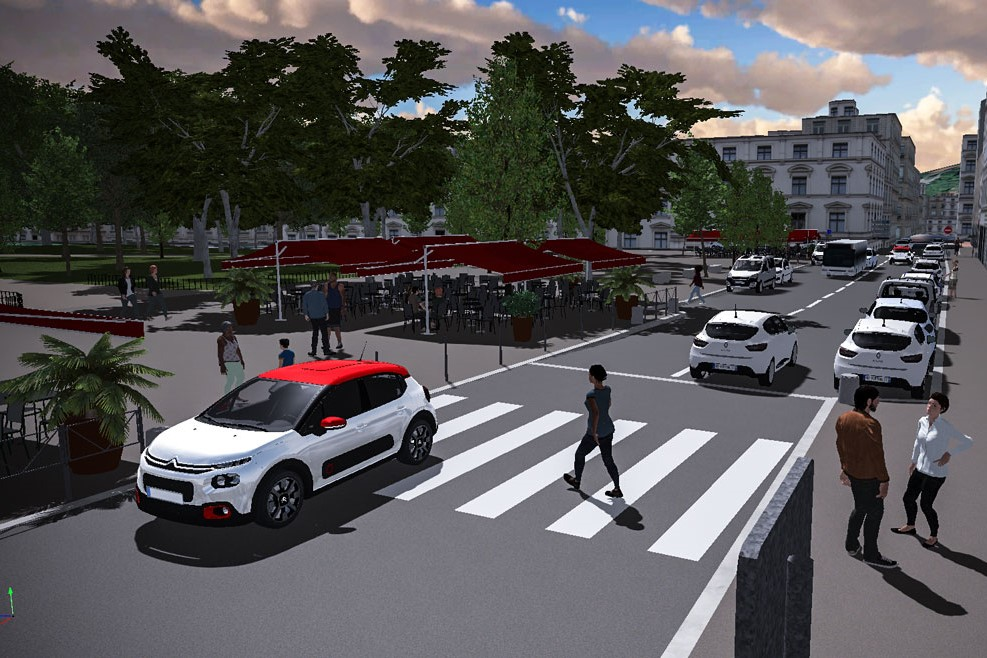
\includegraphics[width=0.5\textwidth]{Simulators/4DV-Sim.jpg}
    \caption{Source: https://www.4d-virtualiz.com/en/automotive-simulator}
\end{figure}

%%%%%%%% AirSIM %%%%%%%%%%
\subsubsection{AirSim}
\textbf{Description:} test

\textbf{Open Source:} Yes

\textbf{Operating System:} Any operating system

\textbf{Game Engine:} Primarily Unreal Engine, but it also offers a prototype version in Unity

\textbf{Pros:}

\textbf{Cons:}

\textbf{Conclusion:}

\begin{figure}[H]
    \centering
    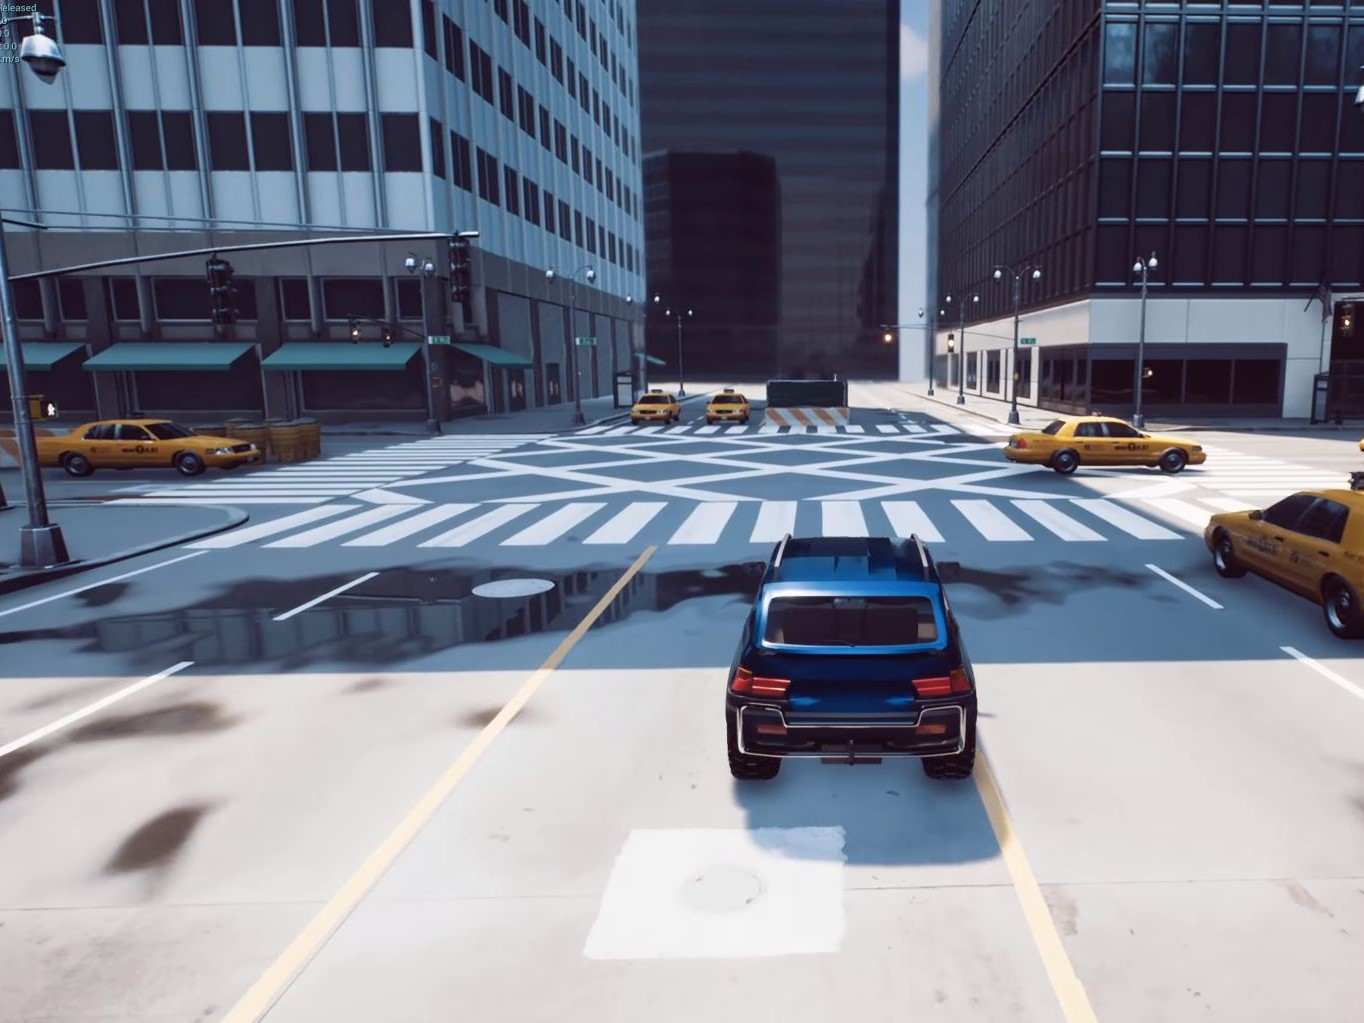
\includegraphics[width=0.5\textwidth]{Simulators/AirSim.JPG}
    \caption{Source: https://microsoft.github.io/AirSim/}
\end{figure}

%%%%%%%% Apollo %%%%%%%%%%
\subsubsection{Apollo}
\textbf{Description:} test

\textbf{Open Source:} Yes

\textbf{Operating System:} Any system that can run Docker

\textbf{Game Engine:} Unity

\textbf{Pros:}

\textbf{Cons:}

\textbf{Conclusion:}



\begin{figure}[H]
    \centering
    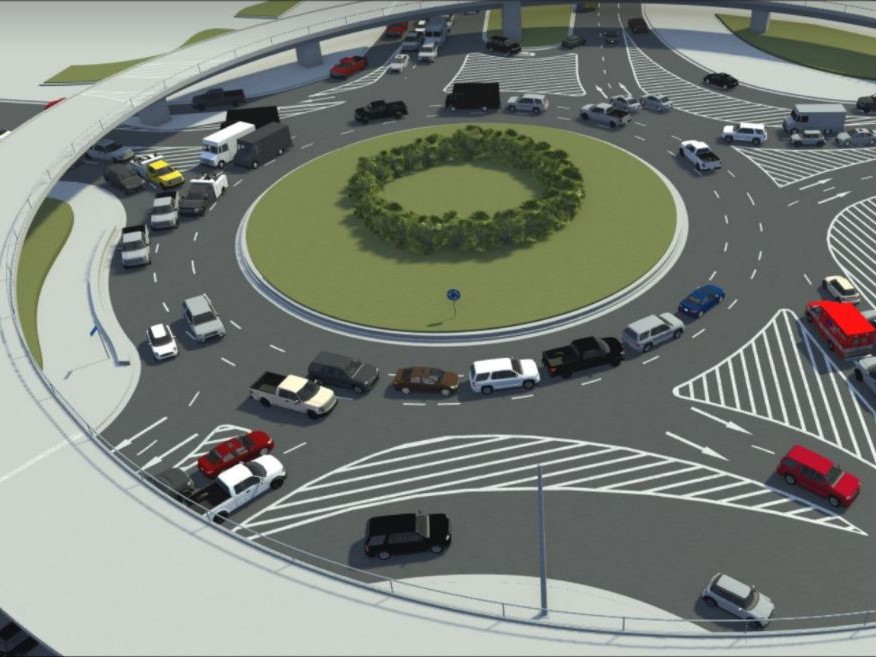
\includegraphics[width=0.5\textwidth]{Simulators/Apollo.JPG}
    \caption{Source: Slide deck from Apollo Game Engine Based Simulation Talk at GDC 2019 - https://bit.ly/2VSzwlF}
\end{figure}

%%%%%%%% Autoware %%%%%%%%%%
\subsubsection{Autoware}
\textbf{Description:} test

\textbf{Open Source:}

\textbf{Operating System:}

\textbf{Game Engine:}

\textbf{Pros:}

\textbf{Cons:}


%%%%%%%% Carla %%%%%%%%%%
\subsubsection{Carla}
\textbf{Description:} test

\textbf{Open Source:}

\textbf{Operating System:}

\textbf{Game Engine:}

\textbf{Pros:}

\textbf{Cons:}


%%%%%%%% CrowdSim3D %%%%%%%%%%
\subsubsection{CrowdSim3D}
\textbf{Description:} test

\textbf{Open Source:}

\textbf{Operating System:}

\textbf{Game Engine:}

\textbf{Pros:}

\textbf{Cons:}

%%%%%%%% Deep Drive %%%%%%%%%%
\subsubsection{Deep Drive}
\textbf{Description:} test

\textbf{Open Source:}

\textbf{Operating System:}

\textbf{Game Engine:}

\textbf{Pros:}

\textbf{Cons:}


%%%%%%%% Donkey Car Simulator %%%%%%%%%%
\subsubsection{Donkey Car Simulator}
\textbf{Description:} test

\textbf{Open Source:}

\textbf{Operating System:}

\textbf{Game Engine:}

\textbf{Pros:}

\textbf{Cons:}


%%%%%%%% Gazebo %%%%%%%%%%
\subsubsection{Gazebo}
\textbf{Description:} test

\textbf{Open Source:}

\textbf{Operating System:}

\textbf{Game Engine:}

\textbf{Pros:}

\textbf{Cons:}


%%%%%%%% LPZRobots %%%%%%%%%%
\subsubsection{LPZRobots}
\textbf{Description:} test

\textbf{Open Source:}

\textbf{Operating System:}

\textbf{Game Engine:}

\textbf{Pros:}

\textbf{Cons:}

%%%%%%%% Marliou %%%%%%%%%%
\subsubsection{Marliou}
\textbf{Description:} test

\textbf{Open Source:}

\textbf{Operating System:}

\textbf{Game Engine:}

\textbf{Pros:}

\textbf{Cons:}

%%%%%%%% MRDS - Microsoft Robotics Developer Studio %%%%%%%%%%
\subsubsection{MRDS - Microsoft Robotics Developer Studio}
\textbf{Description:} test

\textbf{Open Source:}

\textbf{Operating System:}

\textbf{Game Engine:}

\textbf{Pros:}

\textbf{Cons:}


%%%%%%%% rFpro %%%%%%%%%%
\subsubsection{rFpro}
\textbf{Description:} test

\textbf{Open Source:}

\textbf{Operating System:}

\textbf{Game Engine:}

\textbf{Pros:}

\textbf{Cons:}

%%%%%%%% Rigs of Rods %%%%%%%%%%
\subsubsection{Rigs of Rods}
\textbf{Description:} test

\textbf{Open Source:}

\textbf{Operating System:}

\textbf{Game Engine:}

\textbf{Pros:}

\textbf{Cons:}

%%%%%%%% TORCS - The Open Racing Car Simulator %%%%%%%%%%
\subsubsection{TORCS - The Open Racing Car Simulator}
\textbf{Description:} test

\textbf{Open Source:}

\textbf{Operating System:}

\textbf{Game Engine:}

\textbf{Pros:}

\textbf{Cons:}

%%%%%%%% Webots %%%%%%%%%%
\subsubsection{Webots}
\textbf{Description:} test

\textbf{Open Source:}

\textbf{Operating System:}

\textbf{Game Engine:}

\textbf{Pros:}

\textbf{Cons:}